\chapter{均值传递共识算法及算例分析}
\label{cha:Simple}

根据目前提出的众多共识算法,提出了在强连通系统中收敛的简化的共识算法:各个节点通过互相传递等分数据最终收敛于一致值的算法,可以认为去全局加和取平均的分布式演化。

\section{均值传递共识算法}

我们使用有向图的邻接矩阵A来描述其通信拓扑:

\begin{equation}
    \mathbf{A}=\left[a_{i j}\right]_{N \times N}
\end{equation}

$a_{\mathrm{ij}}$为A中的元素:

\begin{equation}
    a_{\mathrm{ij}}=\left\{\begin{array}{ll}
    {1} & {\text { if } j \in N_{i}} \\
    {0} & {\text { Otherwise }}
    \end{array}\right.
\end{equation}

其中N为与i节点相连通的节点集合。

\begin{equation}
    x_{\mathrm{i}}(t)=x_{\mathrm{i}}(t)+u_{\mathrm{i}}(t) \quad i=1,2,3,4 \ldots \ldots, n
\end{equation}

$u_{\mathrm{i}}(t)$为$x_{\mathrm{i}}(t)$的控制变量,服从:

\begin{equation}
    u_{i}(t)=\frac{1}{N_{\mathrm{i}}}\sum_{j=1}^{n} a_{i j}(t)\left[x_{j}(t)-x_{i}(t)\right]
\end{equation}

其中$N_{\mathrm{i}}$为与i节点相连通的节点数。

上述算法的物理含义即:

在第i次迭代过程中,同时对和每个节点相连通的所有节点取平均并赋值给此节点\cite{8706900}。

用过渡矩阵来说就是:Q阵中每个元素为对应邻接矩阵元素除以此节点出度(发出的边的总数)。

\begin{equation}
    q_{i j}=\frac{a_{i j}}{\sum_{k=1}^{N} a_{i k}}
\end{equation}

但此时收敛速度并非最快,在下一章中将会进行优化。


\section{算例}

设想一个四节点机组网络有向图如图~\ref{fig:Directed-graph}:

%去除Visio白边:http://www.mamicode.com/info-detail-2181323.html

\begin{figure}[htbp] % use float package if you want it here
    \centering
    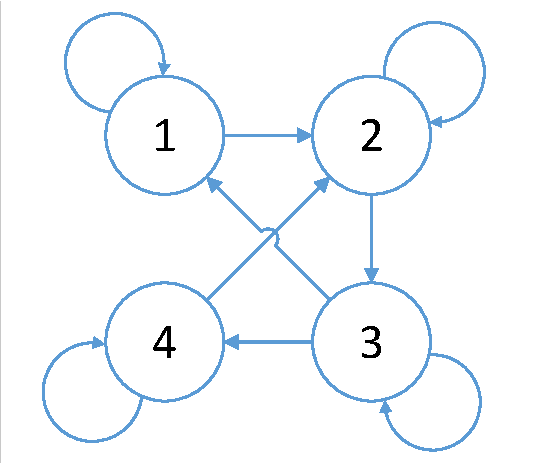
\includegraphics{Directed-graph.pdf}
    \caption{四节点机组网络有向图}
    \label{fig:Directed-graph}
\end{figure}

各节点处机组参数与负荷如表~\ref{tab:example}:

\begin{table}[htbp]
    \centering
%    \resizebox{\textwidth}{!}{%
    \begin{tabular}{@{}ccccc@{}}
    \toprule
    \multicolumn{1}{c}{Node} & $\alpha_{i}(\mathrm{MW})$  & $\beta_{i} \quad\left(\mathrm{MW}^{2} / \mathrm{S}\right)$ & $\gamma_{i}(\mathrm{S})$   & $L_{i}(\mathrm{MW})$    \\ \midrule
    1                        & -1 & 1 & 0.2 & 15.5 \\
    2                        & -2 & 2 & 0.1 & 0    \\
    3                        & -3 & 3 & 0.5 & 15.5 \\
    4                        & -1 & 2 & 0.7 & 0    \\ \bottomrule
    \end{tabular}
%    }缩放表格(字会变得很大)
    \caption{4节点算例机组参数与实时负荷}
    \label{tab:example}
\end{table}

其邻接矩阵为:

\begin{equation}
    A=\left[\begin{array}{cccc}
    {1} & {1} & {0} & {0} \\
    {0} & {1} & {1} & {0} \\
    {1} & {0} & {1} & {1} \\
    {0} & {1} & {0} & {1}
    \end{array}\right]
\end{equation}


\section{简化后的平均值共识算法}

运行附录~\ref{sec:Consensus}中的Python3脚本我们可以得到:

简单取平均后得到过渡矩阵为

\begin{equation}
    Q=\left[\begin{array}{cccc}
    {\frac{1}{2}} & {\frac{1}{2}} & {0} & {0} \\
    {0} & {\frac{1}{2}} & {\frac{1}{2}} & {0} \\
    {\frac{1}{3}} & {0} & {\frac{1}{3}} & {\frac{1}{3}} \\
    {0} & {\frac{1}{2}} & {0} & {\frac{1}{2}}
    \end{array}\right]
\end{equation}

取初值为1,2,3,4迭代10次:

随着迭代各机组的价格曲线如图~\ref{fig:Result-1234}所示。

\begin{figure}[htbp] % use float package if you want it here
    \centering
    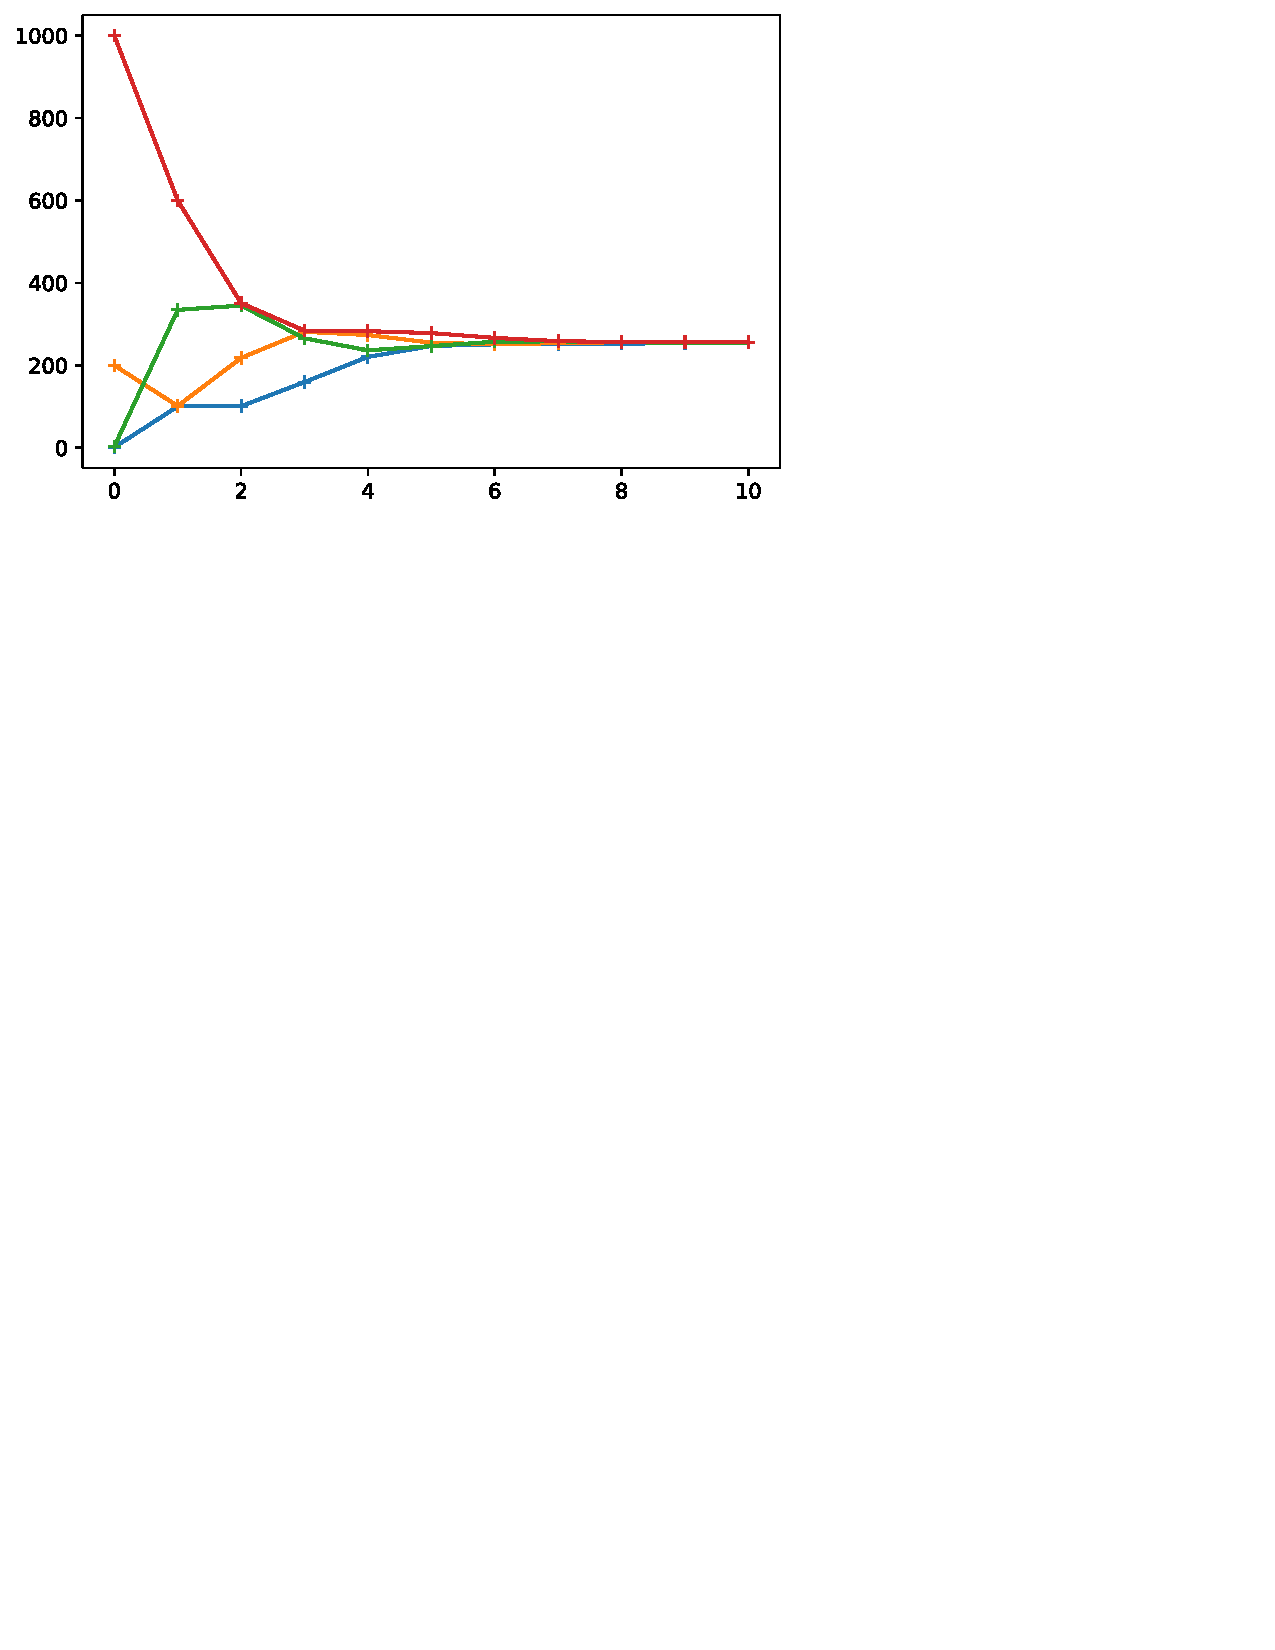
\includegraphics{1234.pdf}
    \caption{初值为1,2,3,4迭代10次的价格曲线}
    \label{fig:Result-1234}
\end{figure}

数据如表~\ref{tab:Result-1234}所示。

\begin{table}[htbp]
    \centering
    \begin{tabular}{|l|l|l|l|l|}
    \hline
    \diagbox{迭代次数}{$X_{i,j}$}{节点编号} %添加斜线表头
       & 0        & 1        & 2        & 3        \\ \hline
    0  & 1        & 2        & 3        & 4        \\ \hline
    1  & 1.5      & 2.5      & 2.666667 & 3        \\ \hline
    2  & 2        & 2.583333 & 2.388889 & 2.75     \\ \hline
    3  & 2.291667 & 2.486111 & 2.37963  & 2.666667 \\ \hline
    4  & 2.388889 & 2.43287  & 2.445988 & 2.576389 \\ \hline
    5  & 2.41088  & 2.439429 & 2.470422 & 2.50463  \\ \hline
    6  & 2.425154 & 2.454925 & 2.461977 & 2.472029 \\ \hline
    7  & 2.44004  & 2.458451 & 2.453054 & 2.463477 \\ \hline
    8  & 2.449246 & 2.455752 & 2.45219  & 2.460964 \\ \hline
    9  & 2.452499 & 2.453971 & 2.454133 & 2.458358 \\ \hline
    10 & 2.453235 & 2.454052 & 2.454997 & 2.456165 \\ \hline
    \end{tabular}
    \caption{初值为1,2,3,4迭代10次各节点价格变化}
    \label{tab:Result-1234}
\end{table}

取初值为1000,0,0,0迭代10次:

随着迭代各机组的价格曲线如图~\ref{fig:Result-1000}所示。

\begin{figure}[htbp] % use float package if you want it here
    \centering
    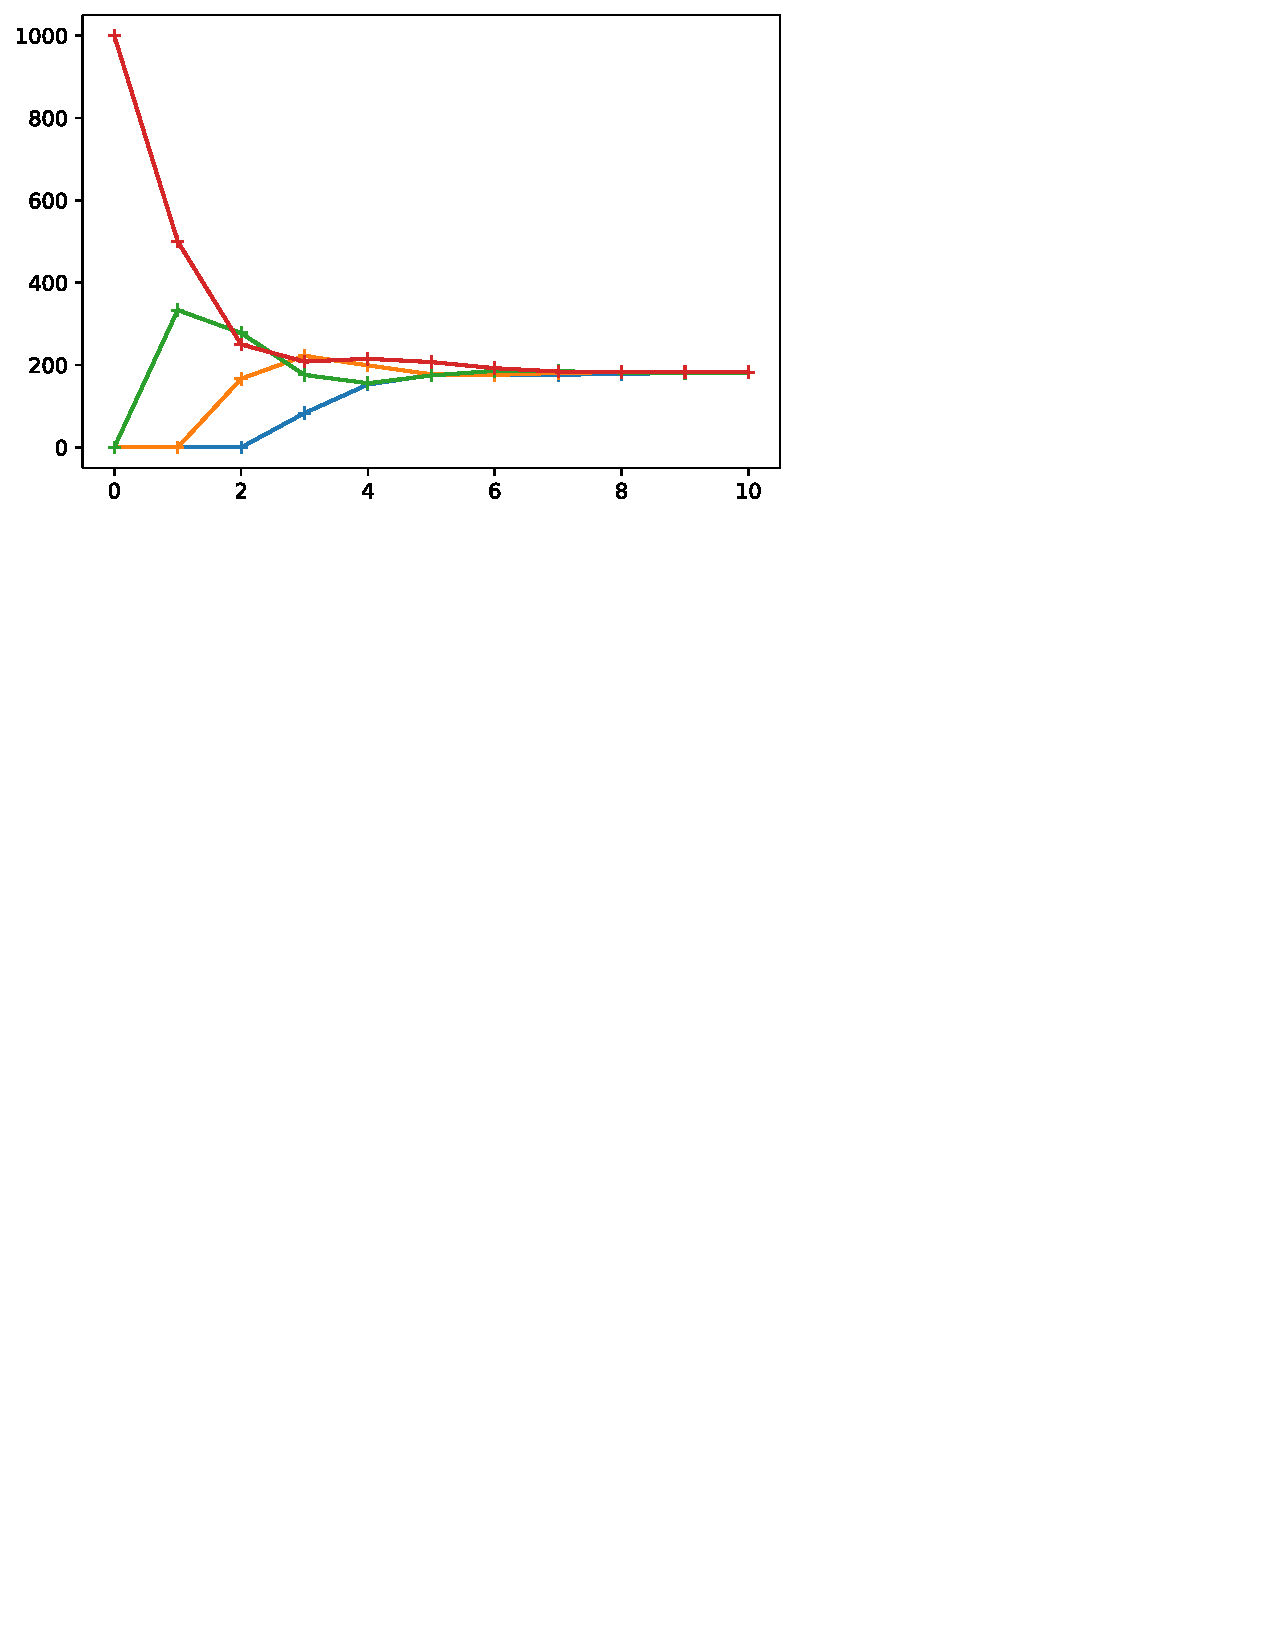
\includegraphics{1000.pdf}
    \caption{初值为1000,0,0,0迭代10次的价格曲线}
    \label{fig:Result-1000}
\end{figure}

数据如表~\ref{tab:Result-1000}所示。

\begin{table}[htbp]
    \centering
    \begin{tabular}{|l|l|l|l|l|}
    \hline
    \diagbox{迭代次数}{$X_{i,j}$}{节点编号} %添加斜线表头
       & 0        & 1        & 2        & 3        \\ \hline
    0  & 0        & 0        & 0        & 1000     \\ \hline
    1  & 0        & 0        & 333.3333 & 500      \\ \hline
    2  & 0        & 166.6667 & 277.7778 & 250      \\ \hline
    3  & 83.33333 & 222.2222 & 175.9259 & 208.3333 \\ \hline
    4  & 152.7778 & 199.0741 & 155.8642 & 215.2778 \\ \hline
    5  & 175.9259 & 177.4691 & 174.6399 & 207.1759 \\ \hline
    6  & 176.6975 & 176.0545 & 185.9139 & 192.3225 \\ \hline
    7  & 176.376  & 180.9842 & 184.978  & 184.1885 \\ \hline
    8  & 178.6801 & 182.9811 & 181.8475 & 182.5864 \\ \hline
    9  & 180.8306 & 182.4143 & 181.038  & 182.7837 \\ \hline
    10 & 181.6225 & 181.7262 & 181.5508 & 182.599  \\ \hline
    \end{tabular}
    \caption{初值为1000,0,0,0迭代10次各节点价格变化}
    \label{tab:Result-1000}
\end{table}

\section{非强连通图反例}

对于一个非强连通图,有向图中的强连通分量会因为单向连接的节点产生全局性的错误迭代结果,需要时刻保证剔除通信错误节点,可以使用握手协议的方法保障双向通信的可靠性。

例如一个10节点系统,1-10号节点取值分别对应为1-10,邻接矩阵A如表~\ref{tab:Error-A}所示。

\begin{table}[htbp]
    \centering
    \begin{tabular}{|l|l|l|l|l|l|l|l|l|l|l|}
    \hline
    \diagbox{i节点编号}{$A_{i,j}$}{j节点编号} %添加斜线表头
       & 1 & 2 & 3 & 4 & 5 & 6 & 7 & 8 & 9 & 10 \\ \hline
    1  & 1 & 1 & 0 & 0 & 1 & 1 & 0 & 1 & 0 & 0  \\ \hline
    2  & 0 & 1 & 1 & 0 & 0 & 0 & 1 & 0 & 1 & 0  \\ \hline
    3  & 1 & 0 & 1 & 1 & 0 & 0 & 1 & 1 & 0 & 1  \\ \hline
    4  & 0 & 1 & 0 & 1 & 0 & 1 & 0 & 0 & 1 & 0  \\ \hline
    5  & 0 & 0 & 0 & 0 & 1 & 0 & 0 & 0 & 0 & 1  \\ \hline
    6  & 0 & 0 & 0 & 0 & 0 & 1 & 0 & 1 & 0 & 0  \\ \hline
    7  & 0 & 0 & 0 & 0 & 0 & 0 & 1 & 0 & 0 & 1  \\ \hline
    8  & 0 & 1 & 0 & 0 & 1 & 1 & 0 & 0 & 0 & 0  \\ \hline
    9  & 0 & 0 & 0 & 0 & 0 & 0 & 0 & 0 & 1 & 0  \\ \hline
    10 & 0 & 0 & 0 & 0 & 1 & 0 & 1 & 0 & 1 & 1  \\ \hline
    \end{tabular}
    \caption{非强连通图反例A矩阵}
    \label{tab:Error-A}
\end{table}

注意表~\ref{tab:Error-A}中9号节点没有办法接收到其他节点的信息,$A_{9,9}=1$是指9号节点能接受到自己的信息,9号节点因此成为错误节点,如果不加握手验证的话,9号节点就成为了害群之马,使得整个网络错误的收敛到9号节点的值9上,而非正确的5.5。

迭代20次曲线如图~\ref{fig:123456-Error}所示。

\begin{figure}[htbp]
    \centering
    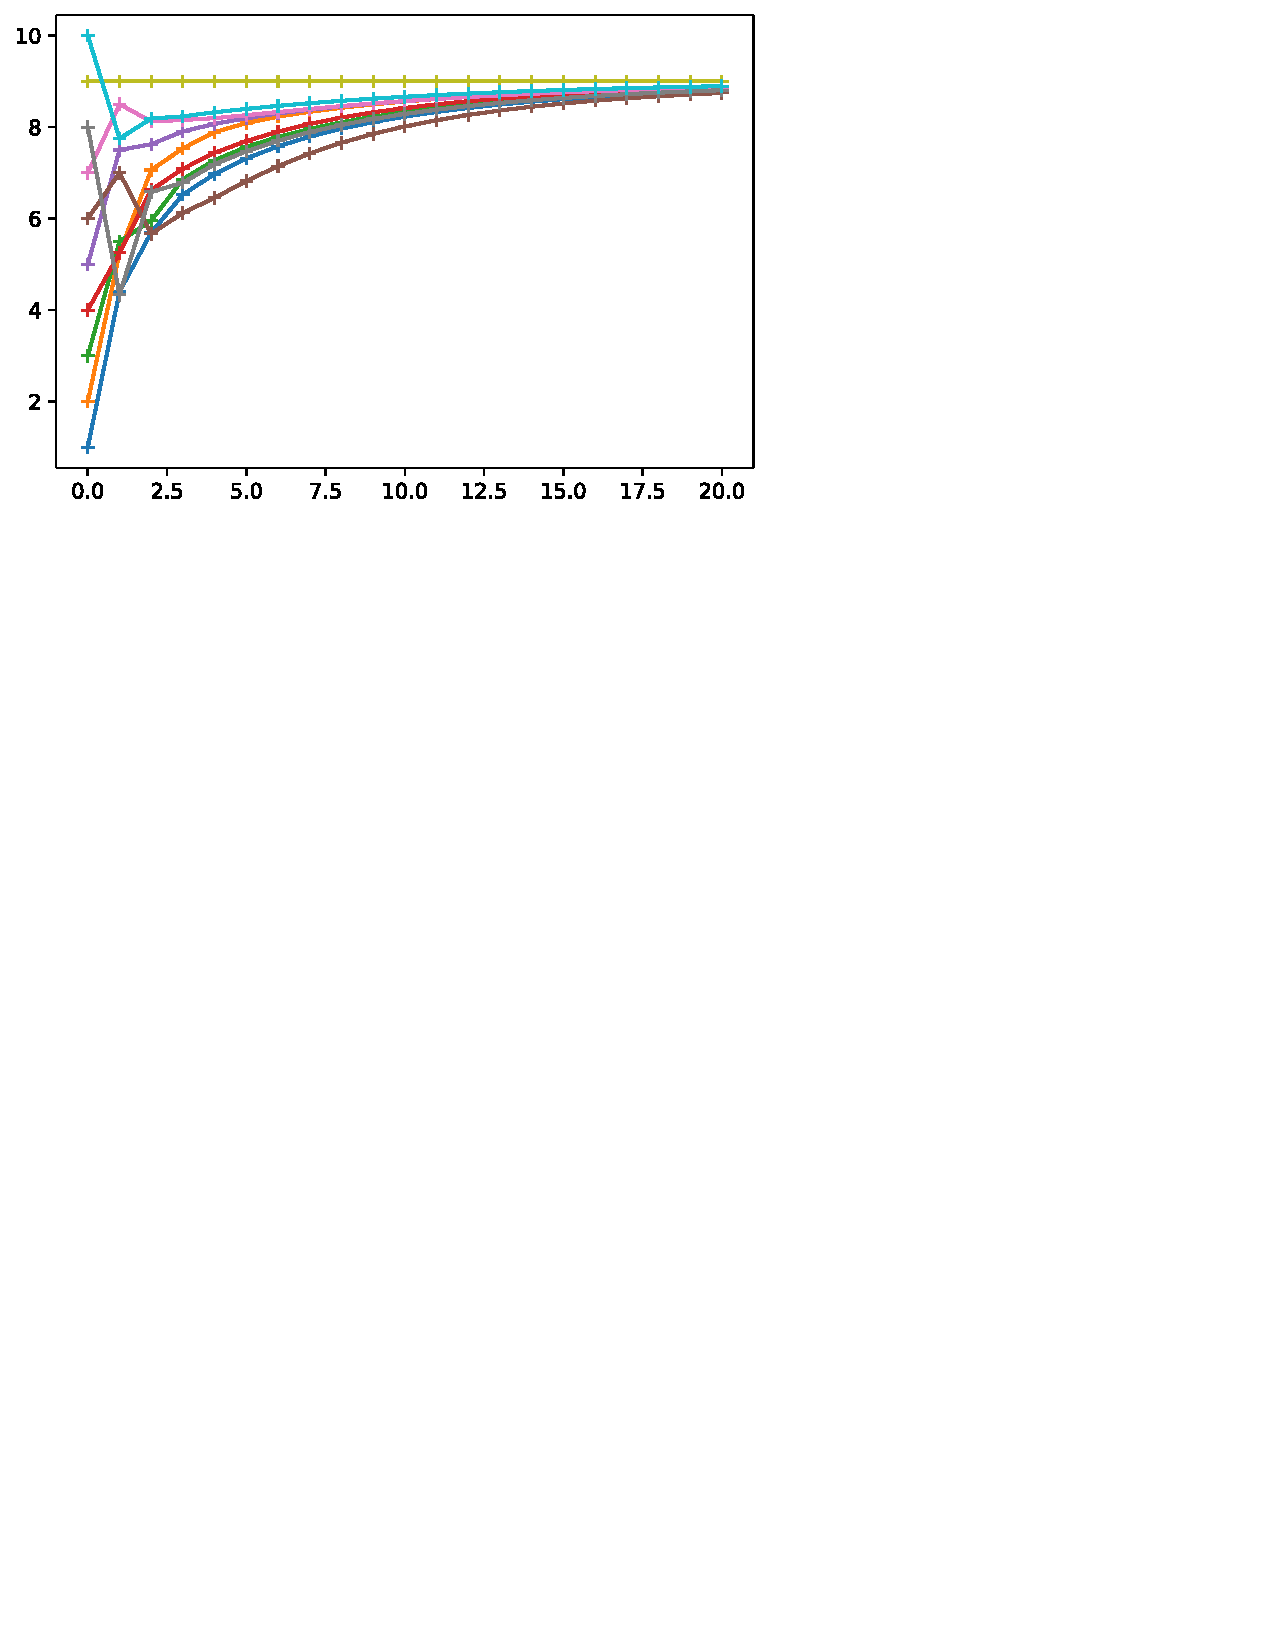
\includegraphics{123456-Error.pdf}
    \caption{非强连通图反例迭代曲线}
    \label{fig:123456-Error}
\end{figure}

数据如表~\ref{tab:123456-Error}所示。

\begin{table}[htbp]
    \centering
    \begin{tabular}{|l|l|l|l|l|l|l|l|l|l|l|}
    \hline
    \diagbox{迭代次数}{$Y_{i,j}$}{节点编号} %添加斜线表头
       & 1    & 2    & 3    & 4    & 5    & 6    & 7    & 8    & 9    & 10    \\ \hline
    0  & 1.00 & 2.00 & 3.00 & 4.00 & 5.00 & 6.00 & 7.00 & 8.00 & 9.00 & 10.00 \\ \hline
    1  & 4.40 & 5.25 & 5.50 & 5.25 & 7.50 & 7.00 & 8.50 & 4.33 & 9.00 & 7.75  \\ \hline
    2  & 5.70 & 7.06 & 5.96 & 6.63 & 7.63 & 5.67 & 8.13 & 6.58 & 9.00 & 8.19  \\ \hline
    3  & 6.53 & 7.54 & 6.86 & 7.09 & 7.91 & 6.13 & 8.16 & 6.78 & 9.00 & 8.23  \\ \hline
    4  & 6.98 & 7.89 & 7.28 & 7.44 & 8.07 & 6.45 & 8.20 & 7.19 & 9.00 & 8.32  \\ \hline
    5  & 7.32 & 8.09 & 7.57 & 7.70 & 8.20 & 6.82 & 8.26 & 7.47 & 9.00 & 8.40  \\ \hline
    6  & 7.58 & 8.23 & 7.78 & 7.90 & 8.30 & 7.15 & 8.33 & 7.70 & 9.00 & 8.46  \\ \hline
    7  & 7.79 & 8.34 & 7.96 & 8.07 & 8.38 & 7.42 & 8.40 & 7.89 & 9.00 & 8.52  \\ \hline
    8  & 7.96 & 8.42 & 8.10 & 8.21 & 8.45 & 7.66 & 8.46 & 8.05 & 9.00 & 8.57  \\ \hline
    9  & 8.11 & 8.50 & 8.23 & 8.32 & 8.51 & 7.85 & 8.52 & 8.18 & 9.00 & 8.62  \\ \hline
    10 & 8.23 & 8.56 & 8.33 & 8.42 & 8.57 & 8.01 & 8.57 & 8.29 & 9.00 & 8.66  \\ \hline
    11 & 8.33 & 8.61 & 8.42 & 8.50 & 8.62 & 8.15 & 8.62 & 8.38 & 9.00 & 8.70  \\ \hline
    12 & 8.42 & 8.66 & 8.49 & 8.57 & 8.66 & 8.27 & 8.66 & 8.46 & 9.00 & 8.73  \\ \hline
    13 & 8.49 & 8.70 & 8.55 & 8.62 & 8.70 & 8.36 & 8.70 & 8.53 & 9.00 & 8.76  \\ \hline
    14 & 8.56 & 8.74 & 8.61 & 8.67 & 8.73 & 8.45 & 8.73 & 8.59 & 9.00 & 8.79  \\ \hline
    15 & 8.61 & 8.77 & 8.66 & 8.71 & 8.76 & 8.52 & 8.76 & 8.64 & 9.00 & 8.81  \\ \hline
    16 & 8.66 & 8.80 & 8.70 & 8.75 & 8.78 & 8.58 & 8.78 & 8.68 & 9.00 & 8.83  \\ \hline
    17 & 8.70 & 8.82 & 8.73 & 8.78 & 8.81 & 8.63 & 8.81 & 8.72 & 9.00 & 8.85  \\ \hline
    18 & 8.74 & 8.84 & 8.77 & 8.81 & 8.83 & 8.67 & 8.83 & 8.75 & 9.00 & 8.87  \\ \hline
    19 & 8.77 & 8.86 & 8.79 & 8.83 & 8.85 & 8.71 & 8.85 & 8.78 & 9.00 & 8.88  \\ \hline
    20 & 8.79 & 8.87 & 8.82 & 8.85 & 8.86 & 8.75 & 8.86 & 8.81 & 9.00 & 8.89  \\ \hline
    \end{tabular}
    \caption{非强连通图反例迭代数据}
    \label{tab:123456-Error}
\end{table}


将其他任意$A_{9,j}$改为1后,就可以变成强连通系统,正常收敛。例如将从节点9到1的有向边连接起来,即令$A_{9,1}=1$其他不变,邻接矩阵A变为如表~\ref{tab:Correct-A}所示。

\begin{table}[htbp]
    \centering
    \begin{tabular}{|l|l|l|l|l|l|l|l|l|l|l|}
    \hline
    \diagbox{i节点编号}{$A_{i,j}$}{j节点编号} %添加斜线表头
       & 1 & 2 & 3 & 4 & 5 & 6 & 7 & 8 & 9 & 10 \\ \hline
    1  & 1 & 1 & 0 & 0 & 1 & 1 & 0 & 1 & 0 & 0  \\ \hline
    2  & 0 & 1 & 1 & 0 & 0 & 0 & 1 & 0 & 1 & 0  \\ \hline
    3  & 1 & 0 & 1 & 1 & 0 & 0 & 1 & 1 & 0 & 1  \\ \hline
    4  & 0 & 1 & 0 & 1 & 0 & 1 & 0 & 0 & 1 & 0  \\ \hline
    5  & 0 & 0 & 0 & 0 & 1 & 0 & 0 & 0 & 0 & 1  \\ \hline
    6  & 0 & 0 & 0 & 0 & 0 & 1 & 0 & 1 & 0 & 0  \\ \hline
    7  & 0 & 0 & 0 & 0 & 0 & 0 & 1 & 0 & 0 & 1  \\ \hline
    8  & 0 & 1 & 0 & 0 & 1 & 1 & 0 & 0 & 0 & 0  \\ \hline
    9  & 1 & 0 & 0 & 0 & 0 & 0 & 0 & 0 & 1 & 0  \\ \hline
    10 & 0 & 0 & 0 & 0 & 1 & 0 & 1 & 0 & 1 & 1  \\ \hline
    \end{tabular}
    \caption{纠正后的强连通图A矩阵}
    \label{tab:Correct-A}
\end{table}

迭代20次曲线如图~\ref{fig:123456-Correct}所示。

\begin{figure}[htbp]
    \centering
    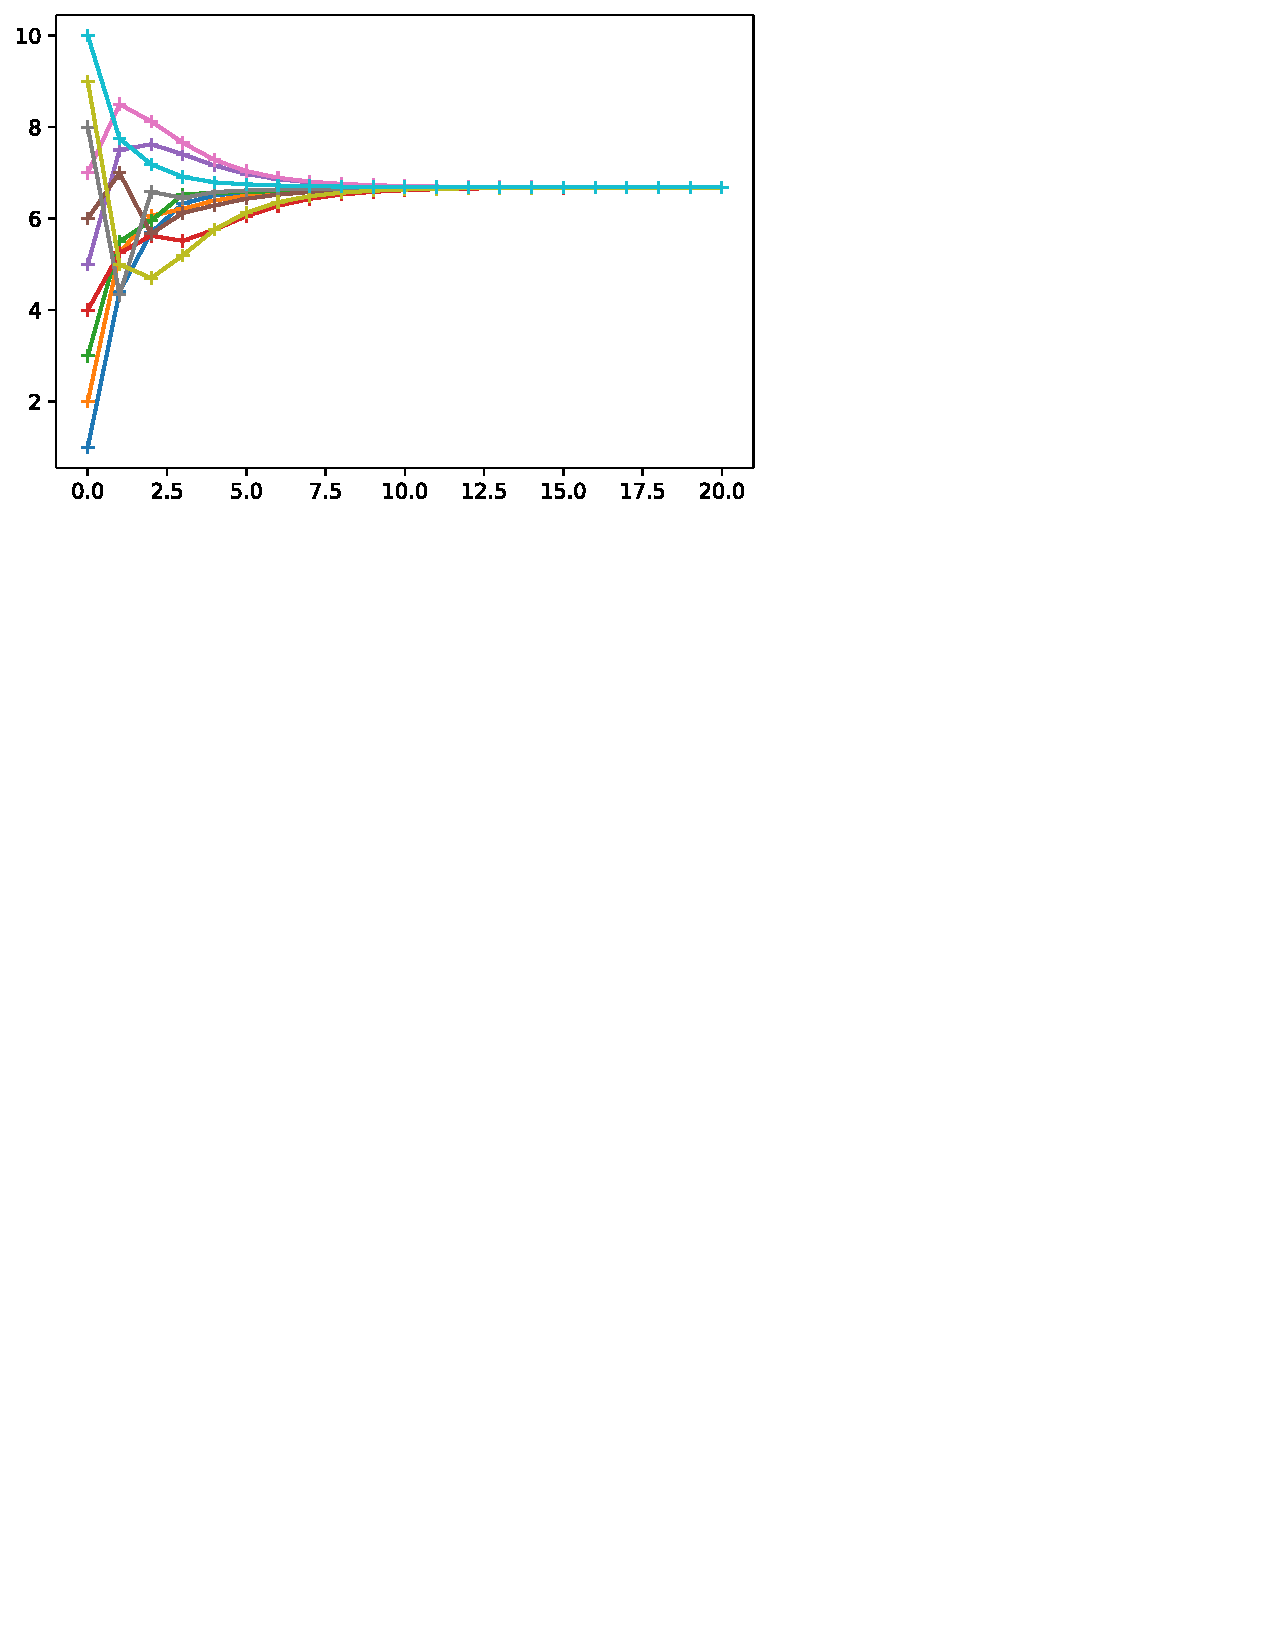
\includegraphics{123456-Correct.pdf}
    \caption{纠正后的强连通图迭代曲线}
    \label{fig:123456-Correct}
\end{figure}

数据如表~\ref{tab:123456-Correct}所示。

\begin{table}[htbp]
    \centering
    \begin{tabular}{|l|l|l|l|l|l|l|l|l|l|l|}
    \hline
    \diagbox{迭代次数}{$Y_{i,j}$}{节点编号} %添加斜线表头
       & 0    & 1    & 2    & 3    & 4    & 5    & 6    & 7    & 8    & 9     \\ \hline
    0  & 1.00 & 2.00 & 3.00 & 4.00 & 5.00 & 6.00 & 7.00 & 8.00 & 9.00 & 10.00 \\ \hline
    1  & 4.40 & 5.25 & 5.50 & 5.25 & 7.50 & 7.00 & 8.50 & 4.33 & 5.00 & 7.75  \\ \hline
    2  & 5.70 & 6.06 & 5.96 & 5.63 & 7.63 & 5.67 & 8.13 & 6.58 & 4.70 & 7.19  \\ \hline
    3  & 6.33 & 6.21 & 6.53 & 5.51 & 7.41 & 6.13 & 7.66 & 6.45 & 5.20 & 6.91  \\ \hline
    4  & 6.50 & 6.40 & 6.56 & 5.76 & 7.16 & 6.29 & 7.28 & 6.58 & 5.76 & 6.79  \\ \hline
    5  & 6.59 & 6.50 & 6.58 & 6.05 & 6.98 & 6.43 & 7.04 & 6.61 & 6.13 & 6.75  \\ \hline
    6  & 6.62 & 6.56 & 6.60 & 6.28 & 6.86 & 6.52 & 6.89 & 6.64 & 6.36 & 6.72  \\ \hline
    7  & 6.64 & 6.60 & 6.63 & 6.43 & 6.79 & 6.58 & 6.81 & 6.65 & 6.49 & 6.71  \\ \hline
    8  & 6.65 & 6.63 & 6.64 & 6.53 & 6.75 & 6.62 & 6.76 & 6.66 & 6.57 & 6.70  \\ \hline
    9  & 6.66 & 6.65 & 6.66 & 6.59 & 6.73 & 6.64 & 6.73 & 6.67 & 6.61 & 6.69  \\ \hline
    10 & 6.67 & 6.66 & 6.67 & 6.62 & 6.71 & 6.65 & 6.71 & 6.67 & 6.64 & 6.69  \\ \hline
    11 & 6.67 & 6.67 & 6.67 & 6.64 & 6.70 & 6.66 & 6.70 & 6.67 & 6.65 & 6.69  \\ \hline
    12 & 6.68 & 6.67 & 6.68 & 6.66 & 6.69 & 6.67 & 6.69 & 6.68 & 6.66 & 6.69  \\ \hline
    13 & 6.68 & 6.68 & 6.68 & 6.67 & 6.69 & 6.67 & 6.69 & 6.68 & 6.67 & 6.68  \\ \hline
    14 & 6.68 & 6.68 & 6.68 & 6.67 & 6.69 & 6.68 & 6.69 & 6.68 & 6.67 & 6.68  \\ \hline
    15 & 6.68 & 6.68 & 6.68 & 6.67 & 6.68 & 6.68 & 6.68 & 6.68 & 6.68 & 6.68  \\ \hline
    16 & 6.68 & 6.68 & 6.68 & 6.68 & 6.68 & 6.68 & 6.68 & 6.68 & 6.68 & 6.68  \\ \hline
    17 & 6.68 & 6.68 & 6.68 & 6.68 & 6.68 & 6.68 & 6.68 & 6.68 & 6.68 & 6.68  \\ \hline
    18 & 6.68 & 6.68 & 6.68 & 6.68 & 6.68 & 6.68 & 6.68 & 6.68 & 6.68 & 6.68  \\ \hline
    19 & 6.68 & 6.68 & 6.68 & 6.68 & 6.68 & 6.68 & 6.68 & 6.68 & 6.68 & 6.68  \\ \hline
    20 & 6.68 & 6.68 & 6.68 & 6.68 & 6.68 & 6.68 & 6.68 & 6.68 & 6.68 & 6.68  \\ \hline
    \end{tabular}
    \caption{纠正后的强连通图迭代数据}
    \label{tab:123456-Correct}
\end{table}


\section{有新节点加入的算例}

整个四节点系统邻接矩阵为:

\begin{equation}
    A=\left[\begin{array}{cccc}
    {1} & {1} & {0} & {0} \\
    {0} & {1} & {1} & {0} \\
    {1} & {0} & {1} & {1} \\
    {0} & {1} & {0} & {1}
    \end{array}\right]
\end{equation}

初始3节点系统迭代10次曲线如图~\ref{fig:123}所示。

\begin{figure}[htbp]
    \centering
    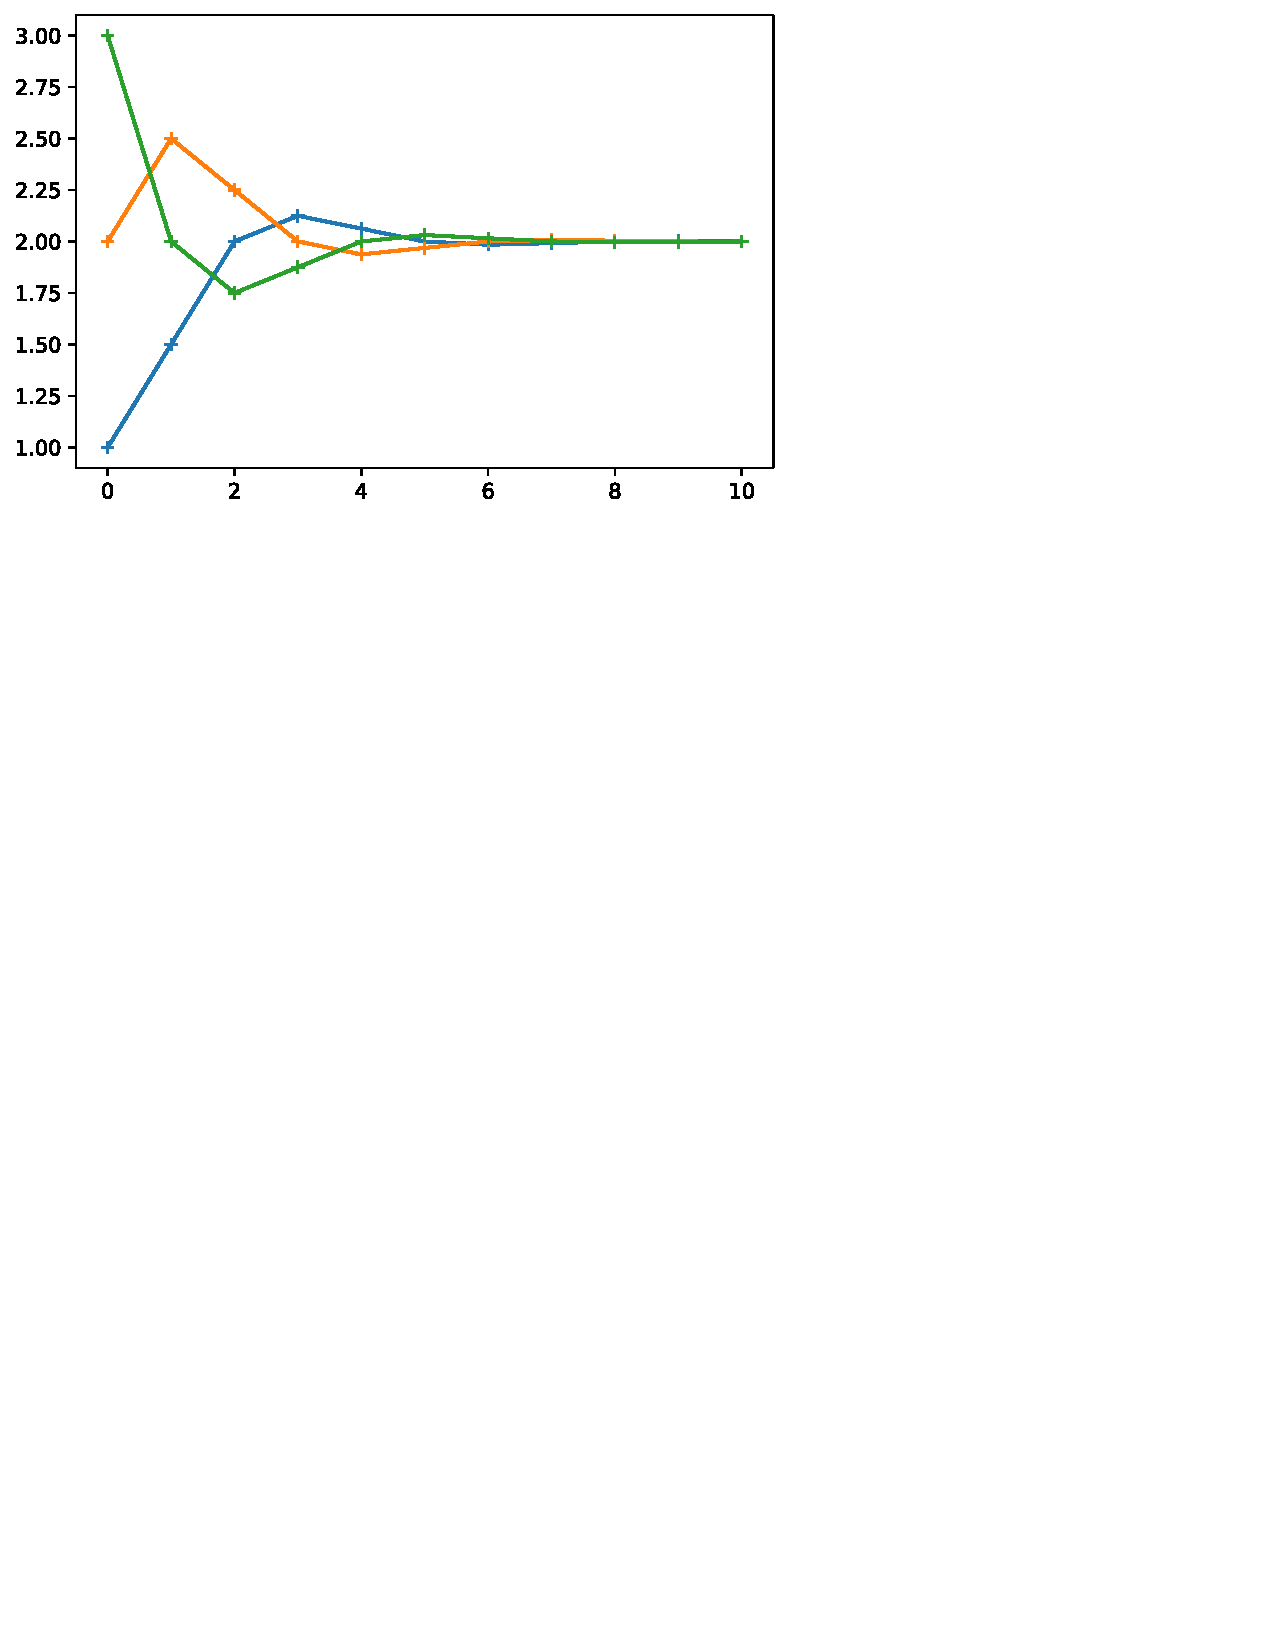
\includegraphics{123.pdf}
    \caption{初始3节点系统迭代10次}
    \label{fig:123}
\end{figure}

数据如表~\ref{tab:123}所示。

\begin{table}[htbp]
    \centering
    \begin{tabular}{|l|l|l|l|}
    \hline
    \diagbox{迭代次数}{$Y_{i,j}$}{节点编号} %添加斜线表头
       & 1    & 2    & 3    \\ \hline
    0  & 1.00 & 2.00 & 3.00 \\ \hline
    1  & 1.50 & 2.50 & 2.00 \\ \hline
    2  & 2.00 & 2.25 & 1.75 \\ \hline
    3  & 2.13 & 2.00 & 1.88 \\ \hline
    4  & 2.06 & 1.94 & 2.00 \\ \hline
    5  & 2.00 & 1.97 & 2.03 \\ \hline
    6  & 1.98 & 2.00 & 2.02 \\ \hline
    7  & 1.99 & 2.01 & 2.00 \\ \hline
    8  & 2.00 & 2.00 & 2.00 \\ \hline
    9  & 2.00 & 2.00 & 2.00 \\ \hline
    10 & 2.00 & 2.00 & 2.00 \\ \hline
    \end{tabular}
    \caption{初始3节点系统迭代过程}
    \label{tab:123}
\end{table}

稳态后加入新节点迭代10次曲线如图~\ref{fig:2224}所示。

\begin{figure}[htbp]
    \centering
    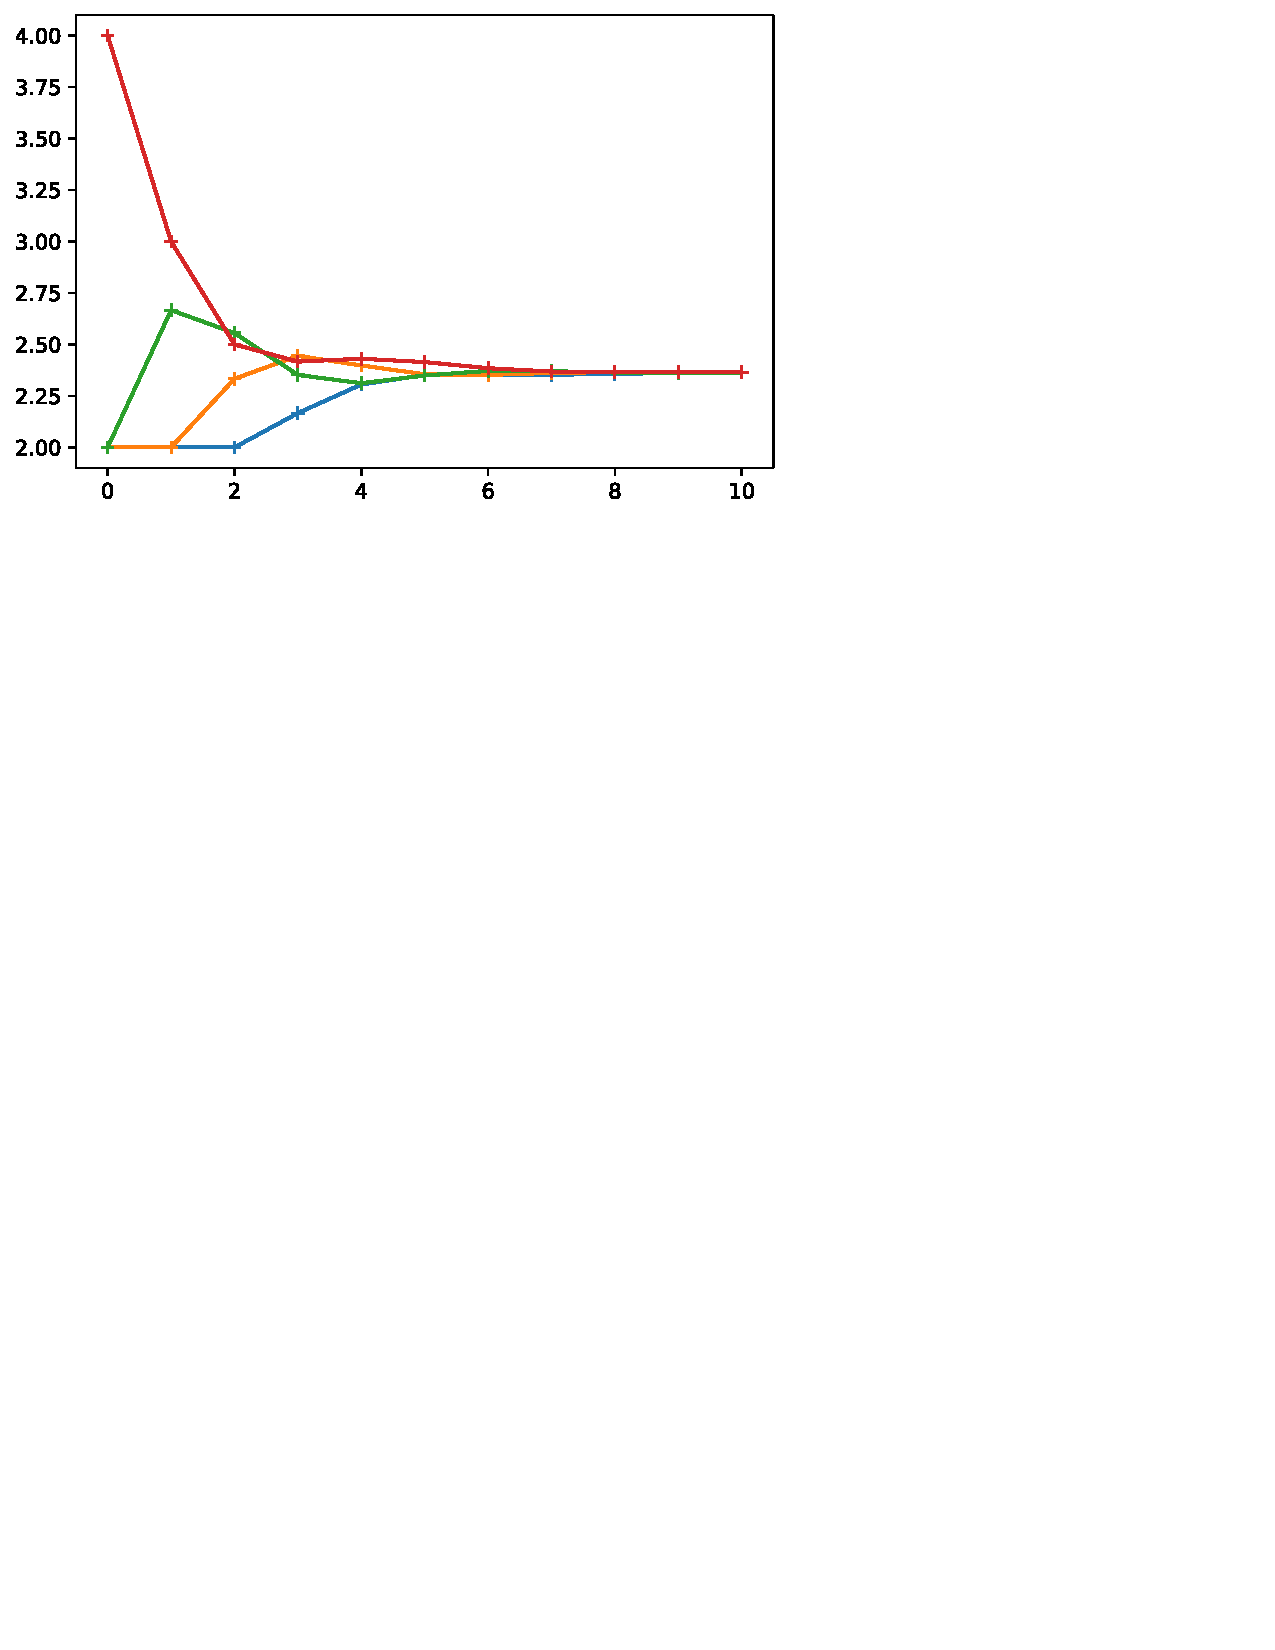
\includegraphics{2224.pdf}
    \caption{纠正后的强连通图迭代曲线}
    \label{fig:2224}
\end{figure}

数据如表~\ref{tab:2224}所示。

\begin{table}[htbp]
    \centering
    \begin{tabular}{|l|l|l|l|l|}
    \hline
    \diagbox{迭代次数}{$Y_{i,j}$}{节点编号} %添加斜线表头
       & 1    & 2    & 3    & 4    \\ \hline
    0  & 2.00 & 2.00 & 2.00 & 4.00 \\ \hline
    1  & 2.00 & 2.00 & 2.67 & 3.00 \\ \hline
    2  & 2.00 & 2.33 & 2.56 & 2.50 \\ \hline
    3  & 2.17 & 2.44 & 2.35 & 2.42 \\ \hline
    4  & 2.31 & 2.40 & 2.31 & 2.43 \\ \hline
    5  & 2.35 & 2.35 & 2.35 & 2.41 \\ \hline
    6  & 2.35 & 2.35 & 2.37 & 2.38 \\ \hline
    7  & 2.35 & 2.36 & 2.37 & 2.37 \\ \hline
    8  & 2.36 & 2.37 & 2.36 & 2.37 \\ \hline
    9  & 2.36 & 2.36 & 2.36 & 2.37 \\ \hline
    10 & 2.36 & 2.36 & 2.36 & 2.37 \\ \hline
    \end{tabular}
    \caption{稳态后加入新节点}
    \label{tab:2224}
\end{table}

整个Illustration过程如图~\ref{fig:123-2224}所示。

\begin{figure}[htbp]
    \centering
    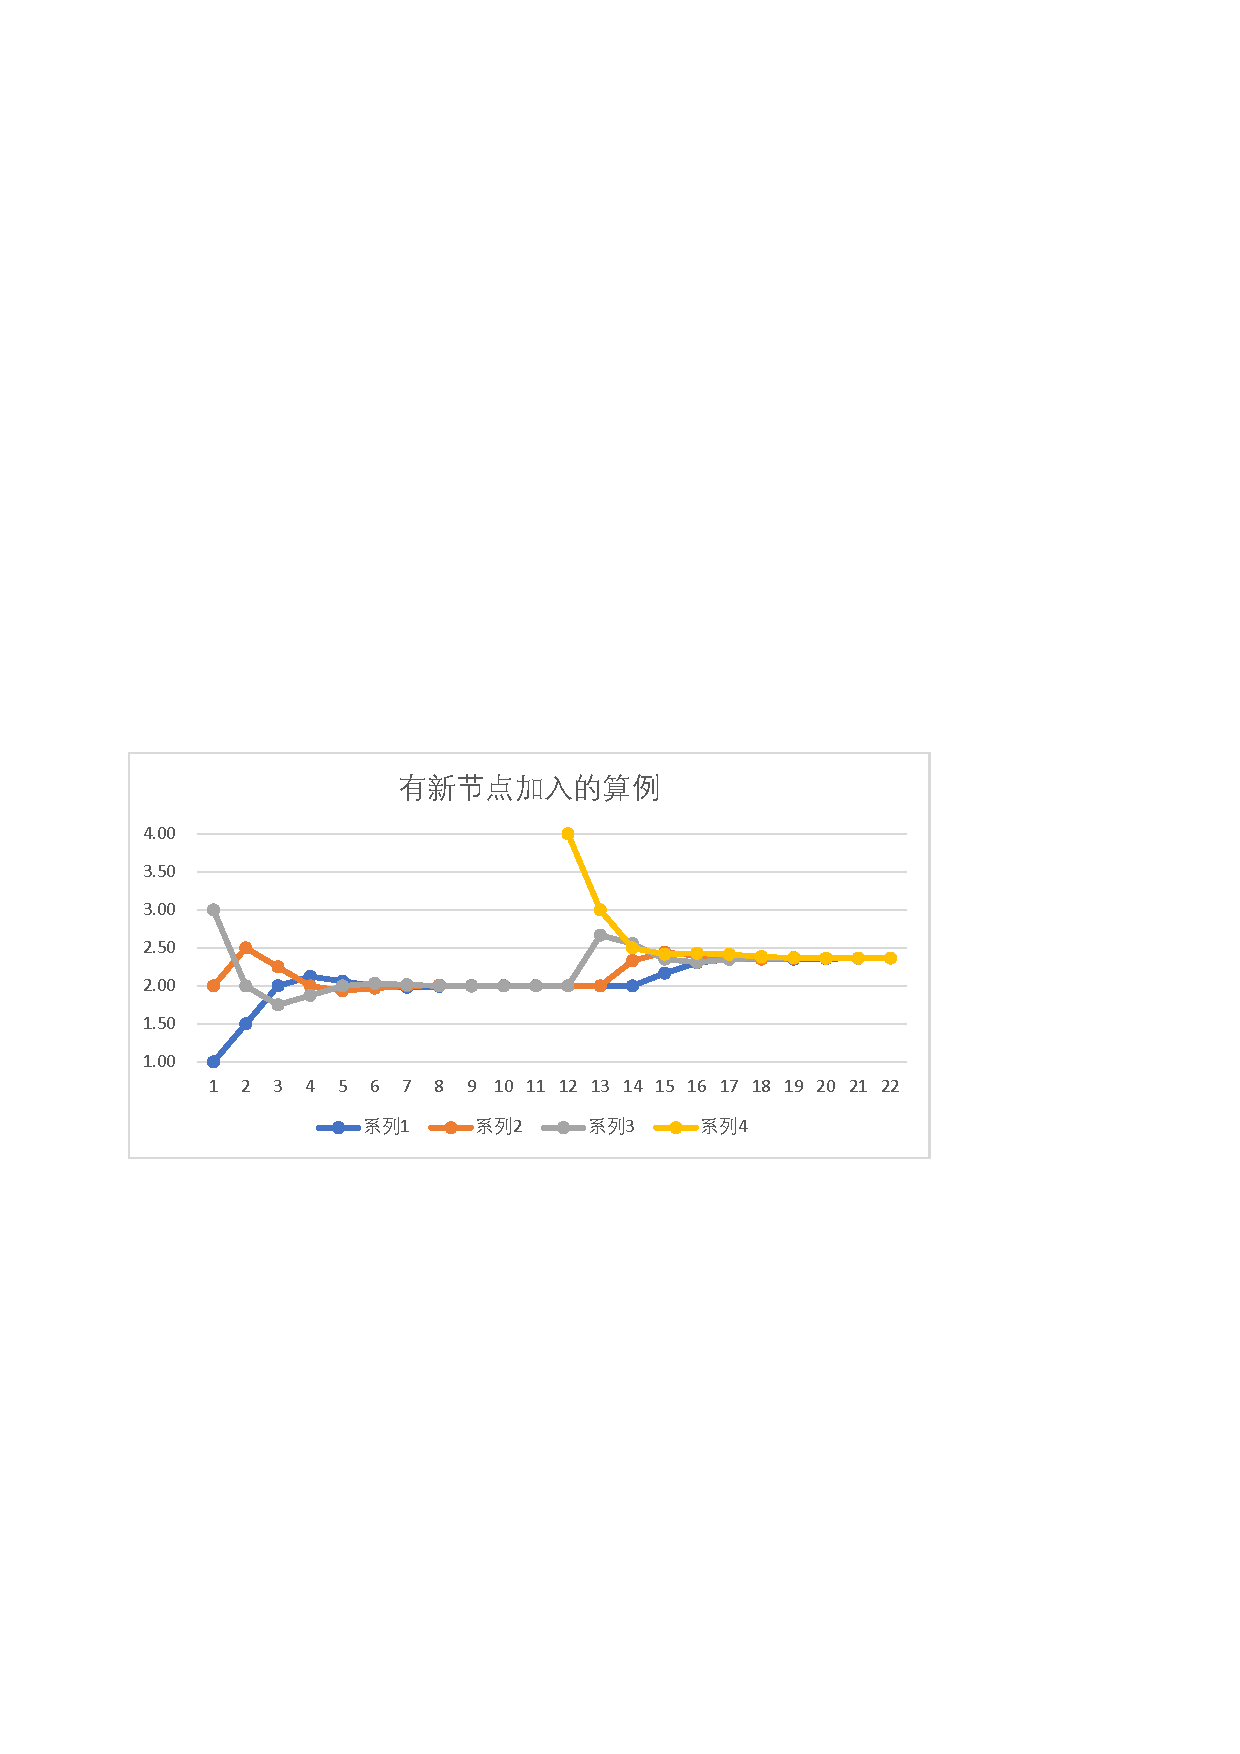
\includegraphics{123-2224.pdf}
    \caption{纠正后的强连通图迭代曲线}
    \label{fig:123-2224}
\end{figure}

\section{动画Illustration设计}

整个Illustration过程如图~\ref{fig:123-2224}所示。

\begin{figure}[htbp]
    \centering
    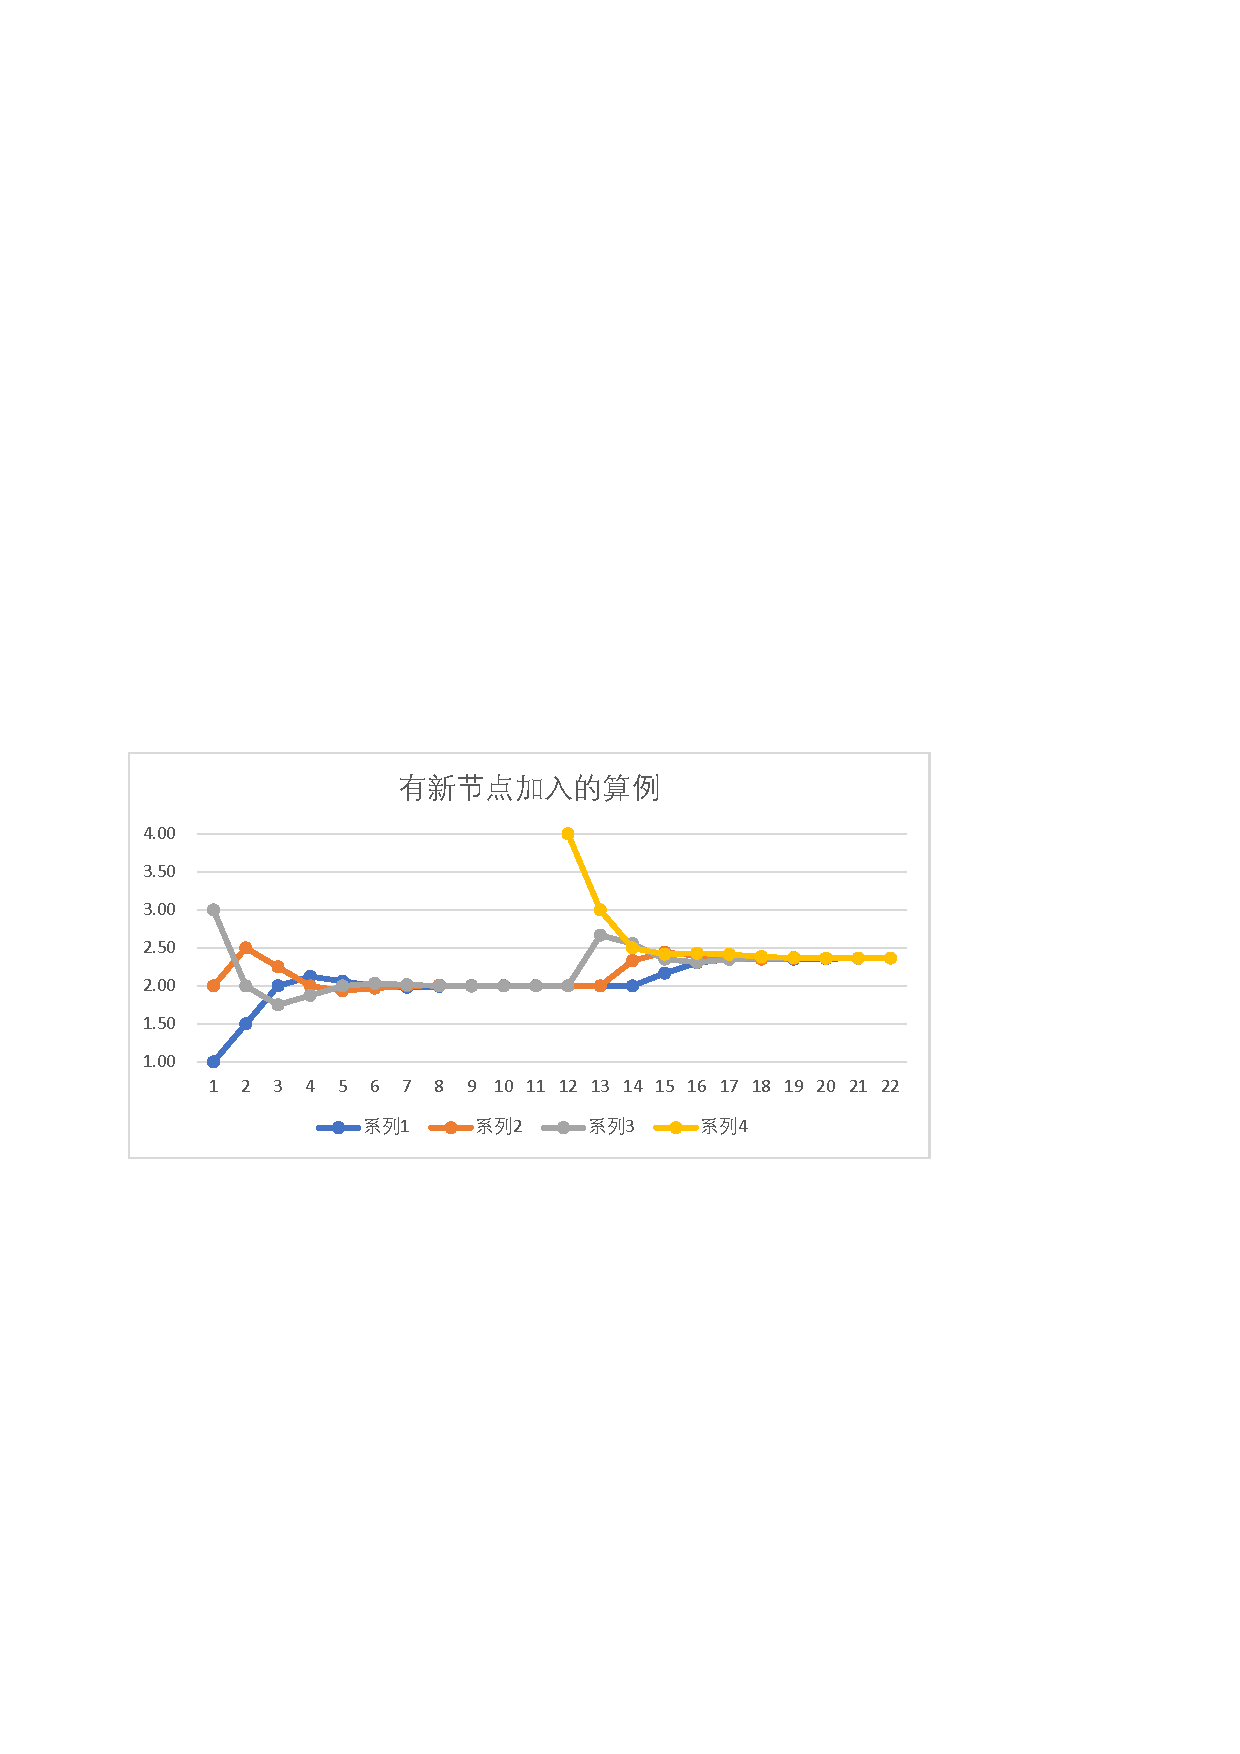
\includegraphics{123-2224.pdf}
    \caption{纠正后的强连通图迭代曲线}
    \label{fig:123-2224}
\end{figure}